\documentclass{fizykalab}

% Ustawienia do tabelki

\wydzial{WI}
\autorjeden{Piotr Karamon}
\autordwa{Hubert Kasprzycki}
\rok{2}
\grupa{12}
\zespol{5}
\temat{Elektroliza}
\nrcwiczenia{35}
\datawykonania{07.11.2023}
\dataoddaniajeden{14.11.2023}
\zwrotdopoprawy{}
\dataoddaniadwa{}
\datazaliczenia{}

\usepackage{amsmath}
\usepackage{amsfonts}
\usepackage{parskip}
\usepackage{multirow}

\newenvironment{conditions}[1][gdzie:]
  {#1 \begin{tabular}[t]{>{$}l<{$} @{${} - {}$} l}}
  {\end{tabular}\\[\belowdisplayskip]}

% \renewcommand{\arraystretch}{1.5}
\newcolumntype{L}[1]{>{\raggedright\let\newline\\\arraybackslash\hspace{0pt}}m{#1}}
\newcolumntype{C}[1]{>{\centering\let\newline\\\arraybackslash\hspace{0pt}}m{#1}}
\newcolumntype{R}[1]{>{\raggedleft\let\newline\\\arraybackslash\hspace{0pt}}m{#1}}

\usepackage[left=1.75cm, right=2cm, top=3cm]{geometry}
\usepackage[labelfont=bf]{caption}

\newcommand{\nm}{\ensuremath{\text{nm}}}
\newcommand{\mm}{\ensuremath{\text{mm}}}
\newcommand{\m}{\ensuremath{\text{m}}}
\newcommand{\vthz}{\ensuremath{\frac{\text{V}}{\text{THz}}}}
\newcommand{\volt}{\ensuremath{\text{V}}}
\newcommand{\Js}{\ensuremath{\text{Js}}}
\newcommand{\echarge}{\ensuremath{1.602 \cdot 10^{-19} \text{C}}}
\newcommand{\s}{\ensuremath{\text{s}}}
\newcommand{\g}{\ensuremath{\text{g}}}
\newcommand{\ampr}{\ensuremath{\text{A}}}
\newcommand{\mampr}{\ensuremath{\text{mA}}}
\newcommand{\mgC}{\ensuremath{\frac{\text{mg}}{\text{C}}}}


\usepackage{natbib}
\usepackage{url}
\begin{filecontents*}{test.bib}
@MISC{elportal-zlacze,
    author = {Michał Kurzela},
    title = {Dioda prostownicza - charakterystyka, oznaczenia, budowa},
    year = {2022},
    note = {[\url{https://elportal.pl/i/2022/09/06/12517-cfe4-1600x0_089-04.jpg}; odwiedzona  14.10.2023]},
    url = {https://elportal.pl/i/2022/09/06/12517-cfe4-1600x0_089-04.jpg}
}
\end{filecontents*}

\begin{document}

\maketitle

\section{Cel ćwiczenia}
Pomiar róznicy mas $\Delta m$ miedzianych elektrod po
przeprowadzeniu elektrolizy, w celu wyznaczenia wartości
równoważnika elektrochemicznego $k$ miedzi, stałej Faradaya
$F$ oraz ładunku elementarnego $e$.

\section{Wstęp teoretyczny}
Charakterystyczną grupę przewodników prądu elektrycznego stanowią elektrolity. Są to
przeważnie wodne roztwory kwasów, zasad i soli, czyli substancji krystalicznych o wiązaniu
jonowym. Przy rozpuszczaniu kryształu wiązania między jonami zostają zerwane i większa
część atomów przechodzi do roztworu w postaci jonów, poruszających się bezładnie
w roztworze.

Gdy do roztworu elektrolitu wstawimy elektrody i dołączymy je do zewnętrznego
źródła prądu stałego o różnicy potencjałów $U$, to ruch jonów staje się uporządkowany.
Kationy zdążają do ujemnej katody, aniony do anody, czyli przez elektrolit płynie prąd. Na
elektrodach jony zostają zobojętnione i stają się zwykłymi atomami lub zgrupowaniami
atomów. Przepływowi prądu towarzyszy więc wydzielanie się substancji na elektrodach.
Proces ten nazywamy elektrolizą. 

Aby naładowany elektrycznie jon mógł zmienić się na elektrodzie na obojętny atom,
musi przepłynąć ładunek równy $w\cdot e$,
gdzie $e$ jest ładunkiem elementarnym elektronu,
natomiast $w$ wartościowością

Liczba atomów wydzielonych na elektrodzie jest stosunkiem ładunku całkowitego
(czyli iloczynu prądu $I$ i czasu $t$) do ładunku pojedynczego jonu 

\begin{equation}
    N = \frac{It}{we}
\end{equation}

Pierwsze prawo elektrolizy Faradaya: Masa $m$ substancji
wydzielonej na elektrodzie jest proporcjonalna
do natężenia prądu $I$ oraz czasu jego
przepływu $t$ (lub po prostu ładunku $Q$):
\begin{equation}
    \label{eq:faraday1}
    m = kIt \quad \text{lub} \quad m = kQ
\end{equation}

Współczynnik proporcjonalności nazywamy
elektrochemicznym równoważnikiem 
substancji i
wynosi on:
\begin{equation}
    \label{eq:k}
    k = \frac{u}{w e N_A}
\end{equation}

Masę powstałych atomów można
obliczyć mnożąc liczbę atomów $N$ 
przez masę 
pojedynczego atomu równą stosunkowi masy molowej $\mu$ do liczby Avogadra $N_A$, czyli 

\begin{equation}
    m = N \frac{\mu}{N_A} = \frac{\mu}{weN_A}It
\end{equation}

Iloczyn $eN_A$
wyraża ładunek potrzebny do wydzielania jednego 
gramorównoważnika
chemicznego substancji. 
Oznacza się go zwykle literą $F$ i nazywa stałą Faradaya.
Z wzoru (\ref{eq:k}) wynika jej związek z wartością $k$,
\begin{equation}
    \label{eq:F}
    F = \frac{u}{wk}
\end{equation}
jej wartość tabelaryczna wynosi $F = e N_A = 96500$ C

Rezultatem elektrolizy roztworu siarczanu miedzi
$\text{CuSO}_4$, przy użyciu elektrod miedzianych,
jest wydzielanie się miedzi na katodzie i ubytek takiej samej masy elektrody dodatniej (anody). 

\section{Opis stanowiska i aparatury pomiarowej}
Stanowisko składało się z:
\begin{itemize}
    \item cyfrowego zasilacza napięcia stałego
    \item amperomierza
    \item trzech elektrod (dwie anody, jedna katoda) w postaci miedzianych płyt
    \item naczynia wypełnionego siarczanem miedzi ($\text{CuSO}_4$)
    \item wody destylowanej i suszarki
    \item wagi elektronicznej
    \item stopera w telefonie
\end{itemize}


\begin{figure}[H]
    \centering
    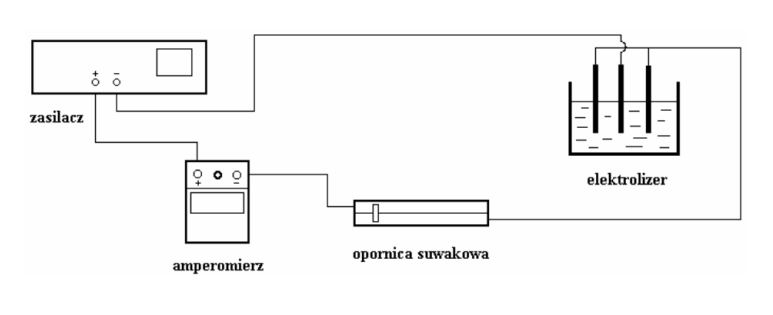
\includegraphics[width=0.75\linewidth]{aparaturka.png}
    \caption{Schematu układu pomiarowego}
\end{figure}


\section{Przebieg doświadczenia}
\begin{enumerate}
    \item Oczyściliśmy elektrody przy użyciu papieru ściernego,
    następnie umyliśmy wodą zwykłą, potem destylowaną.
    \item Płytki osuszyliśmy suszarkami, odczekaliśmy aż
    wystygną, a następnie je zważyliśmy.
    \item Po zanurzeniu elektrod w elektrolicie
    uruchomiliśmy jednocześnie stoper
    oraz zasilanie układu. Amperomierz 
    wskazał natężenie $0,5$A zatem regulacja nie była
    potrzebna.
    \item Odczekaliśmy $29$ minut.
    \item Po tym czasie:
    \begin{enumerate}
        \item wyłączyliśmy zasilanie
        \item wynurzyliśmy elektrody
        \item odczekaliśmy aż elektrolit spłynął z płytek
        \item osuszyliśmy płytki
        \item poczekaliśmy, aż wystygną
        \item ponownie je zważyliśmy
    \end{enumerate}
\end{enumerate}


\section{Wyniki pomiarów}
\begin{table}[H]
    \centering
    \caption{Wyniki pomiarów}
    \begin{tabular}{ll}
        Czas elektrolizy & $t = 29$ min \\
        Natężenie prądu & $I = 0,5A$ \\ \hline
        Masa katody przed elektrolizą & $m_1= 110,387$ g \\
        Masa katody po elektrolizie & $m_2 = 110,683$ g  \\
        Masa wydzielonej miedzi & $m = m_2 - m_1 = 0,296$g \\ \hline
        Masa anod przed elektrolizą &  $M_1 = 190,402$ g \\
        Masa anod po elektrolizie & $M_2 = 190,130$ g \\
        Zmiana masy anod & $M = M_1 - M_2 = 0.272$ g \\
    \end{tabular}
\end{table}

\begin{table}[H]
    \centering
    \caption{Dane określające niepewność przyrządów}
    \begin{tabular}{ll}
         Klasa amperomierza & $0,5$  \\
         Używany zakres amperomierza & $0,75$ A \\
         Niepewność graniczna wagi (znamionowa) & $1$ mg  \\
         Niepewność standardowa wagi  & $u(m) = \frac{\Delta m}{\sqrt{3}} = 0,58$ mg \\
         
    \end{tabular}
\end{table}
\section{Opracowanie wyników}
Na początku wyznaczamy wartość współczynnika elektrochemicznego
ze wzoru (\ref{eq:faraday1}), czyli
\begin{equation*}
    m = kIt \implies  k = \frac{m}{It}
\end{equation*}
\begin{equation*}
    k = \frac{0,296 \g}{0,5 \ampr \cdot 29 \cdot 60 \s} = 
    0,34023 \mgC
\end{equation*}

Korzystając z tej wartości możemy wyznaczyć wartość
stałej Faradaya ze wzoru (\ref{eq:F}), pamiętając, że 
dla $\text{CuSO}_4$ $u = 63,58 \g$ i $w = 2$
\begin{equation*}
    F = \frac{u}{kw} = \frac{63,58 \frac{\g}{\text{mol}} }{0,34023 \mgC \cdot 2} = 
    93436,79  \frac{\text{C}}{\text{mol}}
\end{equation*}


Możemy również obliczyć wartość ładunku elementarnego ze 
wzoru $F = e N_A$
\begin{equation*}
    e = \frac{F} {N_A} = \frac{93436,79
    \frac{\text{C}}{\text{mol}}}
    {6,02214076 \cdot 10^{23} \frac{1}{\text{mol}} } = 
    1,552 \cdot 10^{-19} \text{C} 
\end{equation*}






W przeprowadzanym doświadczeniu istnieją trzy główne źródła niepewności:
\begin{itemize}
    \item niepewność pomiaru natężenia prądu
    \item niepewność pomiaru czasu
    \item niepewność pomiaru wagi płytek miedzianych
\end{itemize}

Niepewność pomiaru czasu zależy głównie od czasu reakcji
człowieka, ale również od czasu uruchomienia zasilania od
momentu wciśnięcia przycisku, zatem ustalamy 
\begin{equation*}
    u(t) = 1 \text{s}
\end{equation*}
Niepewność względna pomiaru czasu wynosi:
\begin{equation*}
    \frac{u(t)}{t} = \frac{1\s}{29 \cdot 60 \s} = 0,058 \%
\end{equation*}

Waga elektroniczna wykorzystana w naszym ćwiczeniu ma 
niepewność graniczną równą $0,001 \g$, jednakże
ważone płytki były podawane wielu zabiegom.
Były czyszczone wodą destylowaną, 
moczone w roztworze, suszone.
z tego powodu
przyjmujemy, że dokładność pomiaru masy płytek wynosi:
\begin{align*}
    u(m) &= 0,015 \g \\
    \frac{u(m)}{m} &= \frac{0,015 \g}{0,296 \g}  = 5,1 \%
\end{align*}

Niepewność analogowego amperomierza określona jest następująco:
\begin{align*}
    \Delta I &= \frac{\text{klasa} \cdot \text{zakres}}{100} 
    = \frac{0,5 \cdot 0,75 \ampr}{100} = 3,75 \mampr \\
    u(I) &= \frac{\Delta I}{\sqrt{3}} = 
    \frac{0,00375 \ampr}{\sqrt{3}} = 2,2 \mampr \\
    \frac{u(I)}{I} &= \frac{2,2\mampr}{500 \mampr} = 0,44 \%
\end{align*}

$k$ jest iloczynem i ilorazem trzech
wielkości mierzonych bezpośrednio zgodnie ze 
wzorem (\ref{eq:faraday1}), a zatem
złożona niepewność względna jest sumą geometryczną względnych niepewności czynników 
\begin{align*}
    \frac{u(k)}{k} &= \sqrt{
        \left[ \frac{u(m)}{m} \right]^2 + 
        \left[ \frac{u(I)}{I} \right]^2 + 
        \left[ \frac{u(t)}{t} \right]^2 
    } =  \sqrt{
        \left( 0,051 \right)^2 + 
        \left( 0,0044  \right)^2 + 
        \left( 0,00058  \right)^2 
    }  = 0,05119 = 5,2 \% \\
    u(k) &= 5,2 \% \cdot 0,296 \g = 0,016 \mgC
\end{align*}

Stała Faradaya obliczana jest z wzoru (\ref{eq:F}) oraz ładunek elementarny obliczany jest z wzoru $F = e N_A$, w których obarczona
niepewnością wartość k jest mnożona (lub dzielona) przez tablicowe wartości $N_A$, $u$ oraz $w$, których
niepewności są pomijalnie małe. Z prawa przenoszenia niepewności względnej wynika, że
niepewności względne $\frac{u(F)}{F}$ oraz $\frac{u(e)}{e}$ są takie same, jak obliczona poprzednio niepewność $\frac{u(k)}{k}$.

\begin{equation*}
    \frac{u(F)}{F} = \frac{u(e)}{e} = 5,2 \%
\end{equation*}

Zatem niepewności bezwzględne stałej Faradaya i
ładunku elementarnego obliczyć można jako:

\begin{align*}
    u(F) &= F \frac{u(k)}{k} = 93436,79  \frac{\text{C}}{\text{mol}} \cdot 5,2 \% = 4900 \frac{\text{C}}{\text{mol}} \\
    u(e) &= e \frac{u(k)}{k} = 1,552 \cdot 10^{-19} \text{C} \cdot 5,2 \% = 0,082 \cdot 10^{-19} \text{C} \\
\end{align*}


\begin{table}[H]
    \centering
    \caption{Zestawienie wyników}
    \begin{tabular}{|c|C{3cm}|C{3cm}|c|c|C{2cm}|}
        \hline
         & wartość tablicowa & wartość wyznaczona w eksperymencie  & różnica  & niepewność  & niepewność względna [\%] \\ \hline
        $k$ [\mgC] & 0,3294 & 0,340 & 0,0106 & 0,016 & 5,2 \\ \hline
        $F$ [$\frac{\text{C}}{\text{mol}}$] & 96500 & 93400 & 3100 & 4900 & 5,2\\ \hline
        $e$ [C] & $1,602 \cdot 10^{-19}$ & $1,552 \cdot 10^{-19}$ & $ 0,05 \cdot 10^{-19}$ & $0,082 \cdot 10^{-19}$ & 5,2 \\ \hline
    \end{tabular}
\end{table}

Wszystkie wyliczone przez nas stałe są zgodne
z wartościami tabelarycznymi, co widać porównując
tabele różnic oraz niepewności. Do stwierdzenia
zgodności nie potrzebowaliśmy niepewności rozszerzonej, 
ponieważ różnice są mniejsze od niepewności pomiarowych.

Zmiana mas anod oraz masa wydzielonej miedzi na katodzie powinny być równe,
jednakże według naszych pomiarów różnią się o $0,024 \g$.
Ustalamy $U(M) = 2 \cdot u(m) = 0,030 \g$, ponieważ 
anody były dwie, a ważono jest osobno, zatem
\begin{align*}
    U(m - M) &= 2 \cdot \sqrt{ \left[ u(m) \right]^2 + \left[ u(M) \right]^2} = 2\sqrt{5\cdot (0,015 \g)^2} = 0,067 \g \\
    |m -M| &= 0,024 \g < U(m - M) 
\end{align*}

Zatem pomimo istnienia różnicy zmiana mas anod oraz masa wydzielonej miedzi są ze sobą zgodne.

\section{Wnioski}
Zgodnie z przewidywaniami, wyniki uzyskane mieszczą się w zakresie wyznaczonej niepewności pomiarowej, przy czym niepewności względne wynoszą $5,2\%$.
Z zadowalającą dokładnością wyznaczyliśmy wartość 
ładunku elementarnego $e$ oraz
stałej Faradaya $F$.
Pomiędzy zmianą mas anod, a masą wydzielonej miedzi istnieje różnica $0,024 \g$ 
jednakże te dwie wartości są ze sobą zgodne.
Głównymi źródłami niepewności były: pomiar masy przy którym trzeba było być bardzo
ostrożnym i uważać by przypadkiem nie zmienić masy płytek oraz 
klasa przyrządów pomiarowych.
\end{document}
 
 
 

